\documentclass{ctexart}
\usepackage[a4paper,top=3cm,bottom=2.7cm,left=2.54cm,right=2.54cm]{geometry}
\usepackage{amsmath,amsfonts,amssymb,amsthm}
\usepackage{mathrsfs}
\usepackage{graphics}
\usepackage{tikz}
\usepackage{multirow}
\usepackage{array}
\usepackage{fancyhdr}
\usepackage{lastpage}
\usepackage{indentfirst}
\usepackage{draftwatermark}         % 所有页加水印
%\usepackage[firstpage]{draftwatermark} % 只有第一页加水印
\SetWatermarkText{半导体物理-期末-模拟}           % 设置水印内容
%\SetWatermarkText{\includegraphics{fig/texlion.png}}         % 设置水印logo
\SetWatermarkLightness{0.85}             % 设置水印透明度 0-1
\SetWatermarkScale{0.3}   
\pagestyle{fancy}
\fancyhf{}
\cfoot{第 \thepage 页 \quad 共 4 页}
\rhead{2024\,—\,2025 学年第一学期\quad }
\lhead{命题:Jack、Z、M \qquad 验题:Z}
\renewcommand{\headrulewidth}{0.7pt}
%\renewcommand{\labelenumi}{\Arabic{enumi}}

\begin{document}

\vspace{1em}
\begin{center}

\textbf{\LARGE NJUIC 《 半导体物理学 》期末模拟考试试卷}
\end{center}

\begin{center}
\begin{tabular}{m{0.3\textwidth} m{0.3\textwidth} m{0.3\textwidth}}
     
     建议时长:\textbf{150分钟} & 考生学号:&考生姓名:
\end{tabular}
\end{center}
\vspace{-0.3cm}
\hrule height 0.5pt
%\noindent
%\rule{\textwidth}{1pt}

\subsection*{一、(30 分)简答}

1. 什么是非平衡载流子?为什么可以引入准费米能级?其含义是什么?\par
2. 什么是空间电荷区?pn结两端不施加偏压时,其载流子漂移和扩散的方向分别是什么? \par
3. pn结的击穿有哪几种状态?简单解释以区别。\par
4. 表面态是什么?它是如何形成的?为什么可能会导致费米能级钉扎效应?\par
5. 什么是金属半导体的欧姆接触?肖特基二极管与同质pn结二极管相比有哪些优点?\par
6. MIS结构中,阈值电压是什么?平带电压是什么?\par
7. 什么是突变型异质结?它与同质的突变型pn结有何不同?什么是应变异质结?\par
8. 为什么可以利用霍尔效应确定半导体的导电类型?霍尔系数是如何定义的?\par

\newpage

\subsection*{二、(7分)}

Z同学自制了一块电阻率为$2.5 \, \Omega \cdot $m 的均匀掺杂的n型材料. 室温下,当材料均匀受到光照射时,在其材料体内均匀产生$\Delta n = \Delta p =2 \times 10^{14} \, \text{cm}^{-3}$的非平衡载流子.\par
1. 给出热平衡状态的判据式.\par
2. 求光照下该材料电阻率的变化量 $ \Delta \rho $.\par
3. 求受光照时该材料电子和空穴的准费米能级相对于原先其费米能级的位置,并做示意图.\par

\vspace{3.5cm}

\subsection*{三、(7分)}



Z同学取用施主浓度为$4.0\times 10^{15} \, \text{cm}^{-3}$的n型硅与Jack提供的镍形成金属-半导体接触. 已知金属镍的功函数为$4.5\, \text{eV}$,硅的电子亲和能为 $4.05\, \text{eV}$. 不考虑表面态的影响,环境温度为30\,$^\circ $C.\par
1. 请做相关计算帮助Z同学判断理想状态下是否形成欧姆接触,并画出该金-半接触的能带图.\par
2. 求施加$0.4 \, \text{V}$反相偏压后的肖特基势垒,并接着问题1画出此时的价带与导带.\par
\vspace{4cm}

\subsection*{四、(6分)}
Jack有一半导体样品交由Z同学检测其导电类型,已知该材料主要由一种载流子导电. Z同学截取了如图所示厚度$c = 0.8 \, \text{mm}$的小片做实验. 室温下,Z同学在$\boldsymbol{x}$方向施加了$1.5 \, \text{V}$电压(对应的电场沿$+\boldsymbol{x}$方向),并测得电流$12\text{mA}$. 若同时在$\boldsymbol{z}$方向施加$0.1\, \text{Wb}/\text{m}^{2}$的磁场(沿$+\boldsymbol{z}$方向),则在$+\boldsymbol{y}$方向可测得$1.3 \, \text{mV}$的电压(对应的电场沿$+\boldsymbol{y}$方向). 请帮助Z同学分析:\par
1. 材料是什么导电类型?\par
2. 载流子的浓度和迁移率是多少?\par


\vspace{-1.2cm}
\begin{figure}[htbp]
    \flushright
    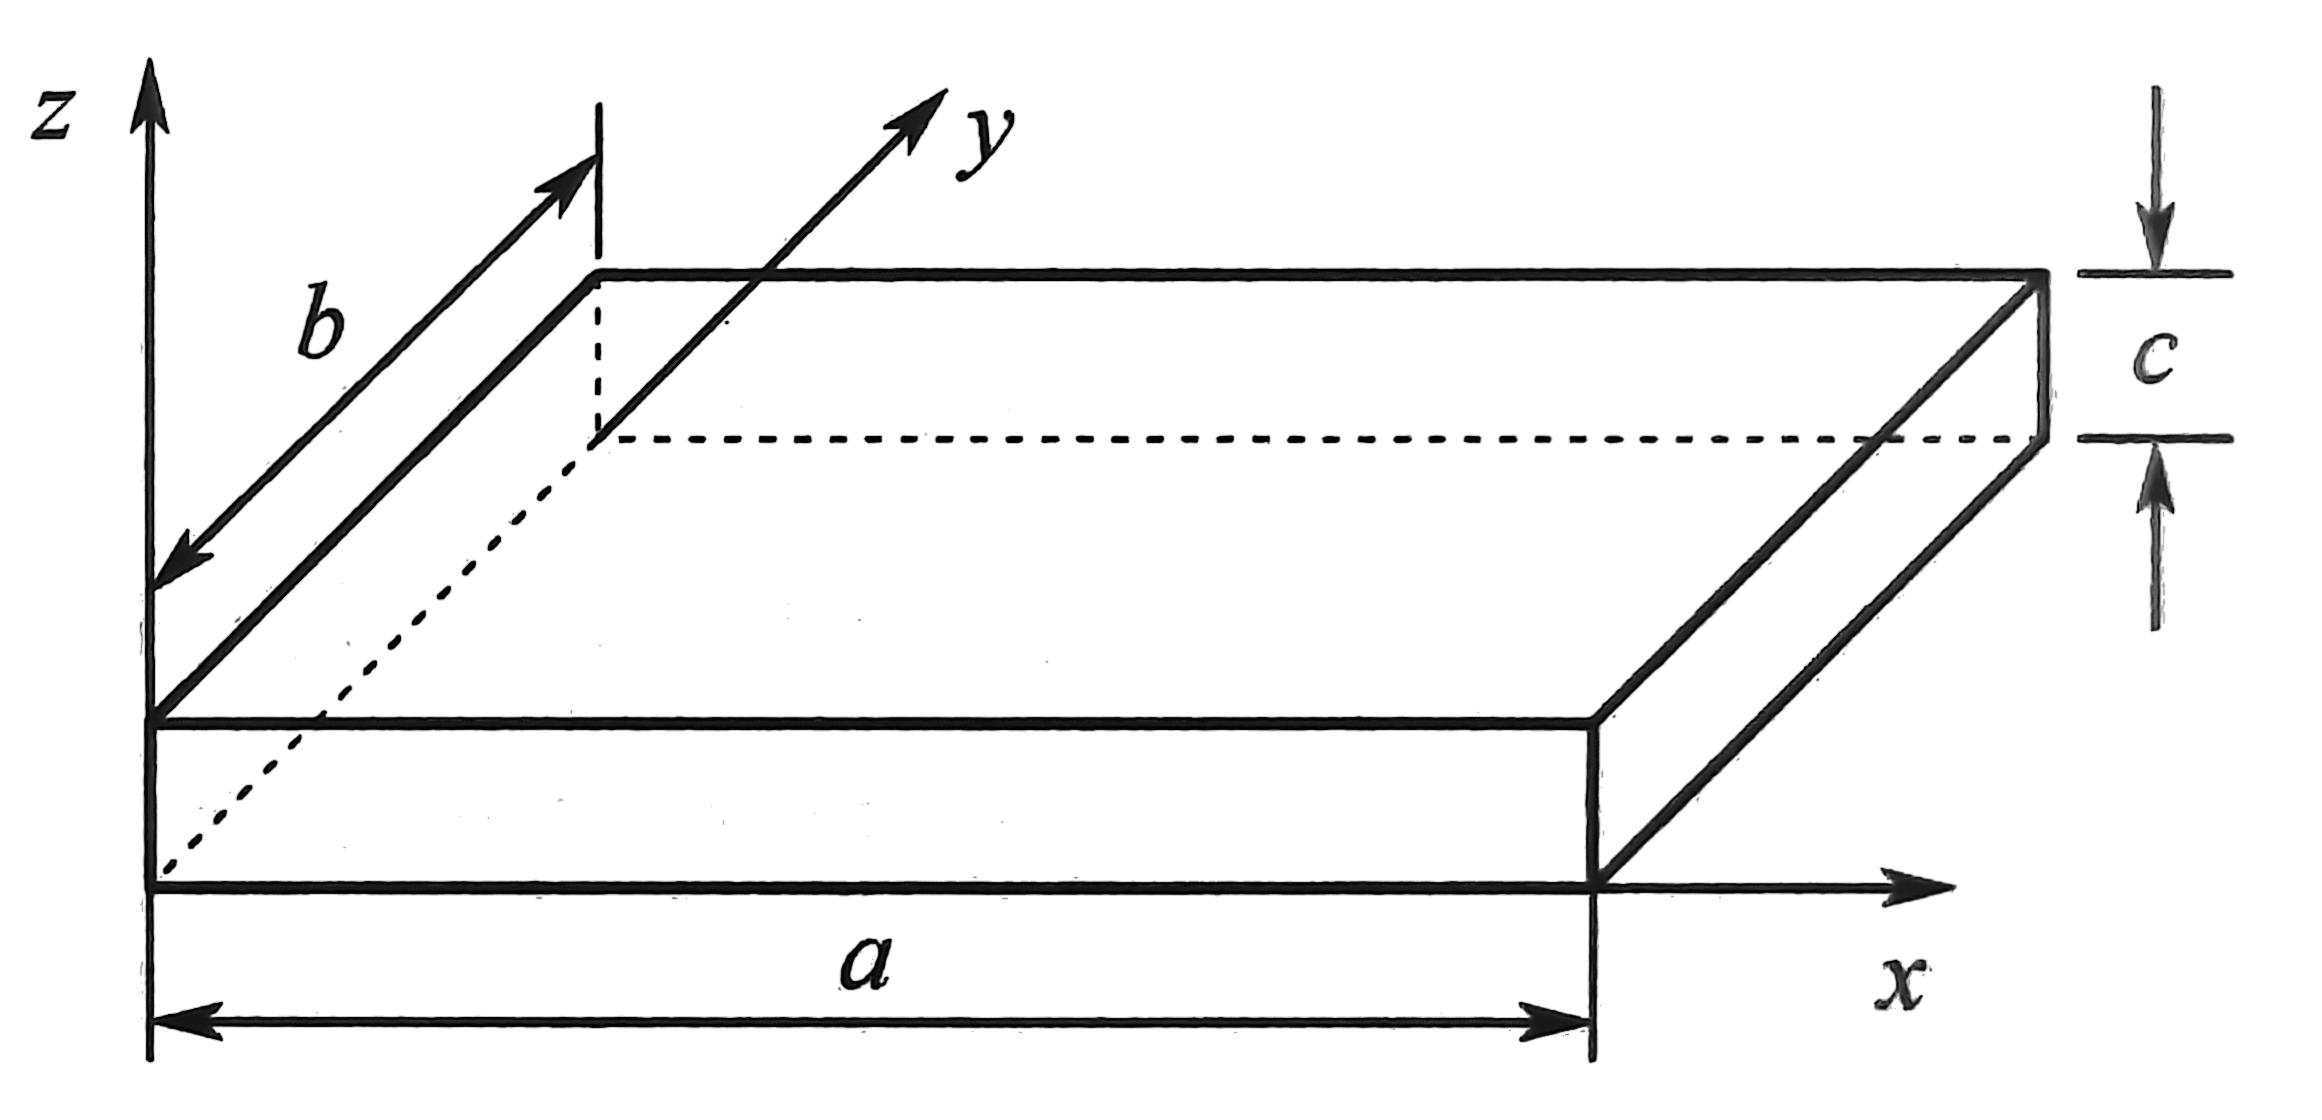
\includegraphics[width=0.45\linewidth]{4.jpeg}
\end{figure}


\newpage
\subsection*{五、(12 分)}
Jack利用题目四中Z同学测定的样品制作得到一理想MIS结构,测定绝缘层的等效氧化硅厚度为 $ t_\text{ox}$ . 在不同的外加电压$V_\text{G}$下,半导体表面状态分别出现积累、耗尽和反型3种类型.\par
1. 分析当出现上述3种状态时所加的外加电压$V_\text{G}$的方向并画出相应的能带图.\par
2. 若室温$T$下,半导体本征载流子浓度为$n_\text{i}$,相对介电常数为$\varepsilon_r$,体内禁带中央与费米能级的差为$qV_\text{B}$. 尝试给出开启电压$V_\text{T}$的表达式,并画出$V_\text{G} = V_\text{T}$时的能带图与电荷分布 $Q(x)$. \par

\vspace{5cm}

\subsection*{六、(16 分)}
Jack有一个硅材料的理想 p$^+$n 突变结,两边杂质浓度分别为 $N_{\text{A} }= 10^{17} \, \text{cm}^{-3} $,$N_{\text{D}}=2 \times 10^{15}\, \text{cm}^{-3}$. 假设材料处在室温$T = 300\, \text{K}$下,空穴寿命 $\tau_{\text{p}} =1\, \mathrm{\mu s} $,电子寿命$\tau_{\text{n}} = 2\, \mathrm{\mu s} $.\par

1. 平衡状态下,计算并绘制该 p$^+$n 结的内建电场分布$ \mathscr{E}_1 (x) $与空间电荷分布 $ Q_1 (x) $,并画出的能带图.\par
2. 给该 p$^+$n 结外加正向偏压$V = 0.5 \, \mathrm{V}$,计算此时的势垒宽度 $ X_{\text{D}}$,并尝试给出n型扩散区少数载流子的连续性方程式(二阶常系数微分方程形式)与相应的边界条件.\par
3. 给该 p$^+$n 结外加反向偏压$V = -0.3 \, \mathrm{V}$,测得反向电流$ I_3 = 10 \, \mathrm{pA}$. 请接着问题1画出此时的能带图与空间电荷分布 $ Q_3 (x) $,并计算问题2中正向电流 $ I_2 $ 的大小.\par


\newpage


\subsection*{七、(12 分)}
对于一杂质浓度为$N_\text{A} = 2.5\times10^{15} \, \text{cm}^{-3}$的p型硅,制作形成一金属-SiO$_2$-Si的MOS结构. 设处在室温环境下,氧化层厚度 $d_0=0.2\mu \text{m}$,金属功函数与硅相同,不考虑界面态影响.\par
1. 求半导体表面恰出现反型层时,空间电荷层中单位面积的电量.\par
2. Z同学测量发现,开启电压的绝对值小于理想模型计算结果. 若差值$|\Delta V_\text{T}| = 1.5\, \text{V}$,请分析氧化层中电荷情况.\par
3. Z同学利用离子注入技术在二氧化硅层中的特定位置注入固定离子,注入离子电荷浓度分布$\rho (x) = k \, x^{-1} e^{-x/d_0} \sin (\pi x/d_0)$,使得该MOS结构平带电压恰为零($x\in [\, 0, d_0],\, x=0$对应金属-氧化层界面). 试计算常数$|k|$,单位$\text{C}\cdot\text{cm}^{-2}$.\par

\vspace{7.5cm}

\subsection*{八、(10 分)}

以真空能级$E_0$为基准,一n型锗材料其禁带宽度$E_\text{g1}=0.67\,$eV、功函数$W_1=4.31\,$eV、电子亲和能$X_1=4.13\,$eV,又有一p型砷化镓材料其禁带宽度$E_\text{g2}=1.42\,$eV、功函数$W_2=5.32\,$eV、电子亲和能$X_2=4.07\,$eV. 现Z同学被要求用两材料接触制作一理想pn突变结.\par

1. 画出该pn结不施加电压时的能带图,并标注出上述相关能带结构参数.\par
2. 计算导带阶与价带阶的值并在问题1所作图中做标注.\par
3. 计算该pn结的内建电势$V_\text{D}$,并在问题1所作图中标注出交界面两侧材料各自的内建电势.\par
4. 已知介电常数$\varepsilon_\text{Ge}>\varepsilon_\text{GaAs}$,试定性画出该pn结内建电场分布$\mathscr{E}(x)$.\par


\newpage
\thispagestyle{empty}
\begin{center}
    \subsection*{常用参数及参考公式}
\end{center}

{
    
    1. 室温下硅材料相关参数:\par
    \qquad 本征载流子浓度:$n_\text{i} = 1.02 \times 10^{10} \, \text{cm}^{-3}$ \par
    \qquad 相对介电常数:$\varepsilon_\text{rs} = 11.9$ \par
    \qquad 导带底有效态密度:$N_\text{c} = 2.8\times 10^{19} \, \text{cm}^{-3}$ \par
    \qquad 电子迁移率:$1450\, \text{cm}^2 / (\text{V}\cdot \text{s})$ \par
    \qquad 空穴迁移率:$\, \, \, 500\, \text{cm}^2 / (\text{V}\cdot \text{s})$ \par

    \vspace{0.5cm}
    
    2. 载流子的计算公式:\par
    
    \vspace{0.1cm}
    
    \qquad \qquad $n_0 = N_\text{c} \exp \left( -\dfrac{E_\text{c} - E_\text{F}}{kT}\right) = n_\text{i} \exp \left( -\dfrac{E_\text{i} - E_\text{F}}{kT}\right)$ \par
    
    \vspace{0.1cm}
    
    \qquad \qquad $p_0 = N_\text{v} \exp \left( -\dfrac{E_\text{F} - E_\text{v}}{kT}\right) = n_\text{i} \exp \left( -\dfrac{E_\text{F} - E_\text{i}}{kT}\right)$ \par 
    
    \vspace{0.1cm}
    
    \qquad \qquad $n_0 p_0 = n_\text{i}^2$ \par
    
    \vspace{0.5cm}
    
    3. 导电性能:\par
    \qquad 杂质半导体电导率:$ \sigma = n q \mu_\text{n} + p q \mu_\text{p}$ \par
    \qquad 附加电导率:$ \Delta \sigma =\Delta  n q \mu_\text{n} + \Delta  p q \mu_\text{p}$ \par

    \vspace{0.5cm}
    
    4. 耗尽区相关公式(其中$\varepsilon_0 = 8.854 \times 10^{-14} \; \text{F} \cdot \text{cm}^{-1} $)\par
    \vspace{0.1cm}
    \qquad 耗尽区势垒高度与宽度的关系:$|V| = \dfrac{q N_\text{A}}{2\varepsilon_r \varepsilon_0} x_\text{p}^2 + \dfrac{q N_\text{D}}{2\varepsilon_r \varepsilon_0} x_\text{n}^2$ \par
    \qquad 耗尽区电场分布:
    \vspace{-0.3cm}
    \[
        \mathscr{E} (x) = 
        \begin{cases}
            -\cfrac{q N_\text{A}}{\varepsilon_r \varepsilon_0} (x + x_\text{p}) & \text{if }\; x \in (-x_\text{p},\, 0\, ] \\
            
            \cfrac{q N_\text{D}}{\varepsilon_r \varepsilon_0} (x - x_\text{n}) & \text{if }\; x \in [\, 0,\, x_\text{n})
        \end{cases}
    \]
    \vspace{-0.5cm} 
    \par
    \qquad 耗尽区单位面积:$ Q = -q N_\text{A} x_\text{p} $或$ Q = q N_\text{D} x_\text{n} $\par
    
    \vspace{0.5cm}

    5. 绝缘层单位面积电容:$C_0 = \cfrac{\varepsilon_r \varepsilon_0}{d_0}$(氧化硅的相对介电常数$\varepsilon_{r0} = 3.9$)
    
}
\end{document}
